%
% Firstprint.tex
%
% LulzBot mini User Manual
%
% Copyright (C) 2014 Aleph Objects, Inc.
%
% This document is licensed under the Creative Commons Attribution 4.0
% International Public License (CC BY-SA 4.0) by Aleph Objects, Inc.
%
%
%
%%%% Not used in the Mini manual, this has now been replaced by the quick start guide. The following section can be enabled then updated for usage with the Mini. %%%%


\section{Set Temperature}
\index{temperature}
%Make sure to first read the instructions for using the Printrun software. Connect to the printer as described in the Printrun software section
%%% XXX pageref going to \label not \section (page \pageref{Installing Printrun}).
The Mini 3D printer ships with a small length of ABS filament from our testing prior to shipping. The filament will need to be removed before proceeding. In order to do so set the hot end to 230C. Make sure that the \texttt{Monitor Printer} (Found in the upper middle portion of the Pronterface window) check box is selected. Once the hot end has reached 230C, gently squeeze both the idler screws and the plastic clip together and pull upwards to release the idler. Rotate the idler counter clockwise, exposing the filament and the filament drive (hobbed bolt). Remove the filament by hand by gently pulling it out. Allow more time for the filament to soften if the filament cannot be removed easily.

Set the hot end and print surface for ABS or PLA plastic and turn both on. The temperature settings for ABS should be set at \texttt{230°C} for the hot end and \texttt{85°C} for print surface; for PLA they should be set at \texttt{185°C} for the hot end and \texttt{55°C} for print surface. These temperatures work well for filament sourced from LulzBot, however you may need to adjust the temperature a degree or two depending on the filament source, color and type. Click the \texttt{Motors Off} button.
\glossary{Idler}{Refers to parts using a bearing (usually a 608ZZ) to add tension in belts or to add pressure against a rolling surface.}
\section{Load Filament}
\index{filament}
\index{hot end}

Once the hot end is heated to the correct temperature you will now need to load the plastic filament into the extruder.
\begin{figure}[hbt]
\centering
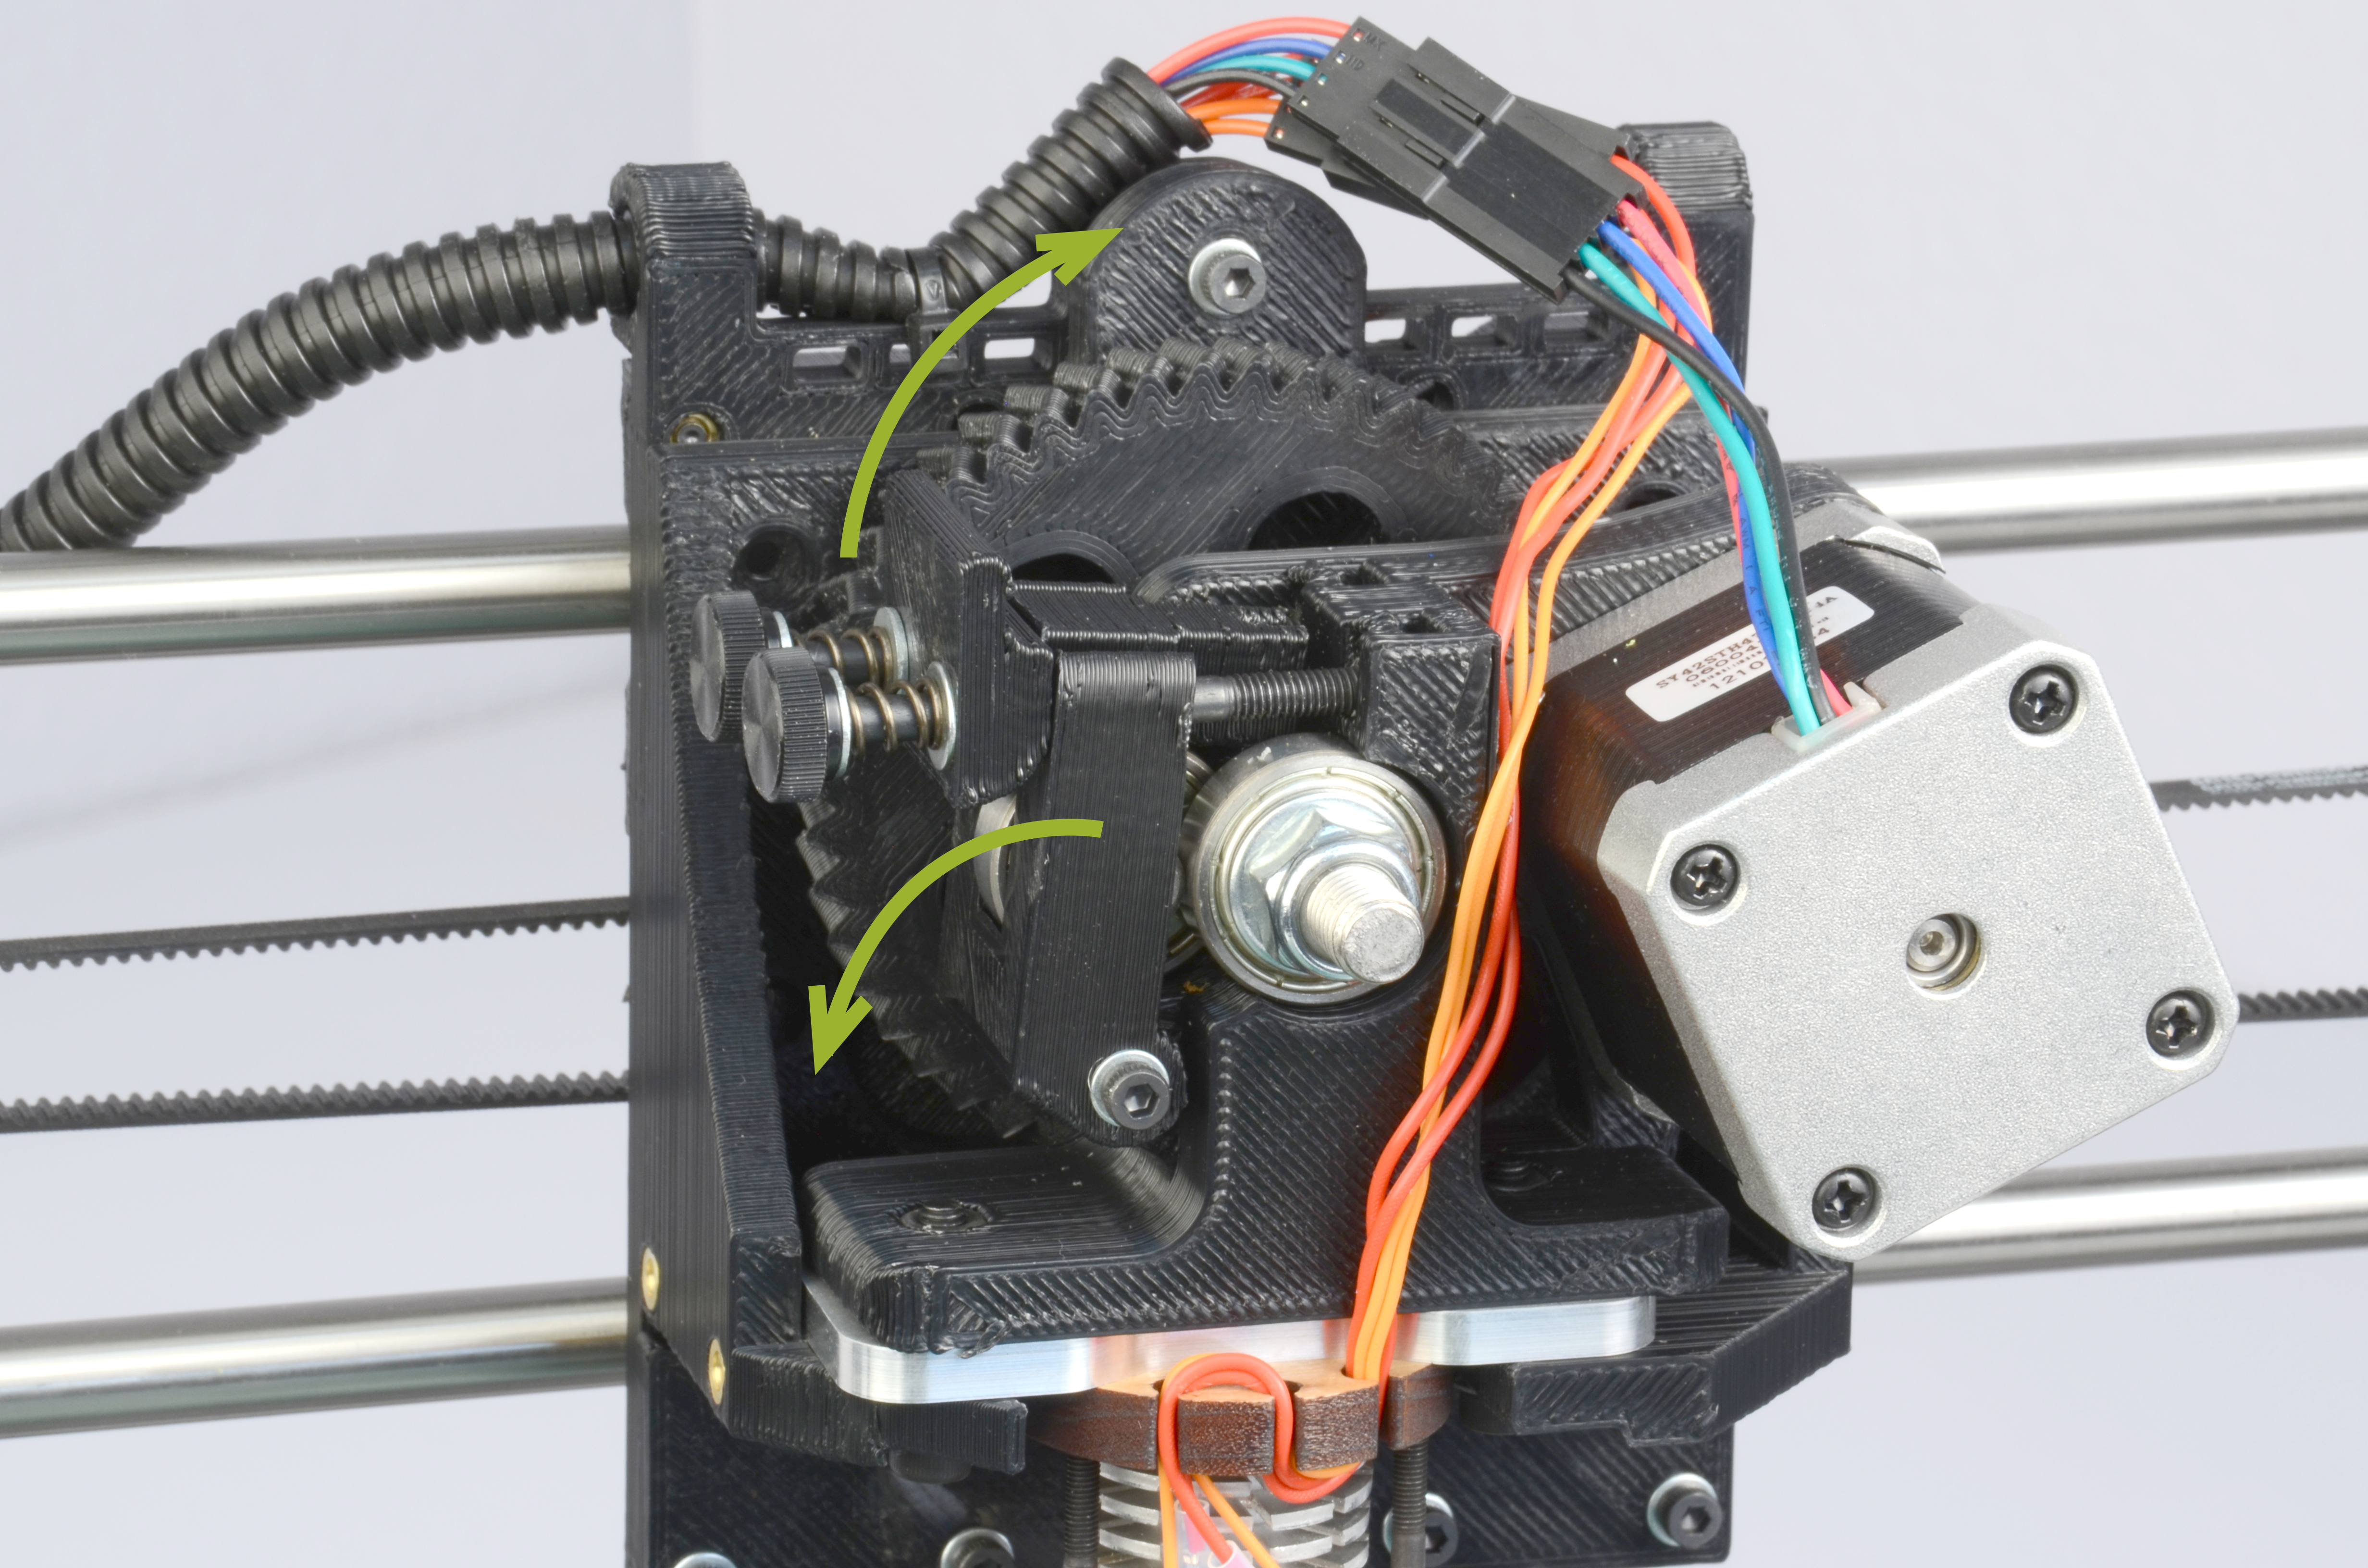
\includegraphics[keepaspectratio=true,angle=0,height=0.4\textheight,width=1.0\textwidth]{extruder_idler_release.JPG}
\caption{Extruder idler release}
\label{fig:extruder_idler_release}
\end{figure}
% update feed hole picture.
Gently squeeze both the idler screws and the plastic clip together and pull upwards to release the idler (Fig. \ref{fig:extruder_idler_release}, page \pageref{fig:extruder_idler_release}). The idler screws can be loosened if necessary. The idler can be rotated downwards allowing access to the hobbed bolt and filament feed hole(Fig. \ref{fig:extruder_filament_slot}, page \pageref{fig:extruder_filament_slot}). If the extruder has a small section of filament already loaded, you will need to remove the filament once the extruder idler has been opened, by gently pulling out the filament by hand once the hot end has reached extrusion temperature. From the previously installed filament reel, feed the end of the plastic filament into the filament feed hole
(Fig. \ref{fig:extruder_filament_slot}, page \pageref{fig:extruder_filament_slot}).
\begin{figure}[hbt]
\centering
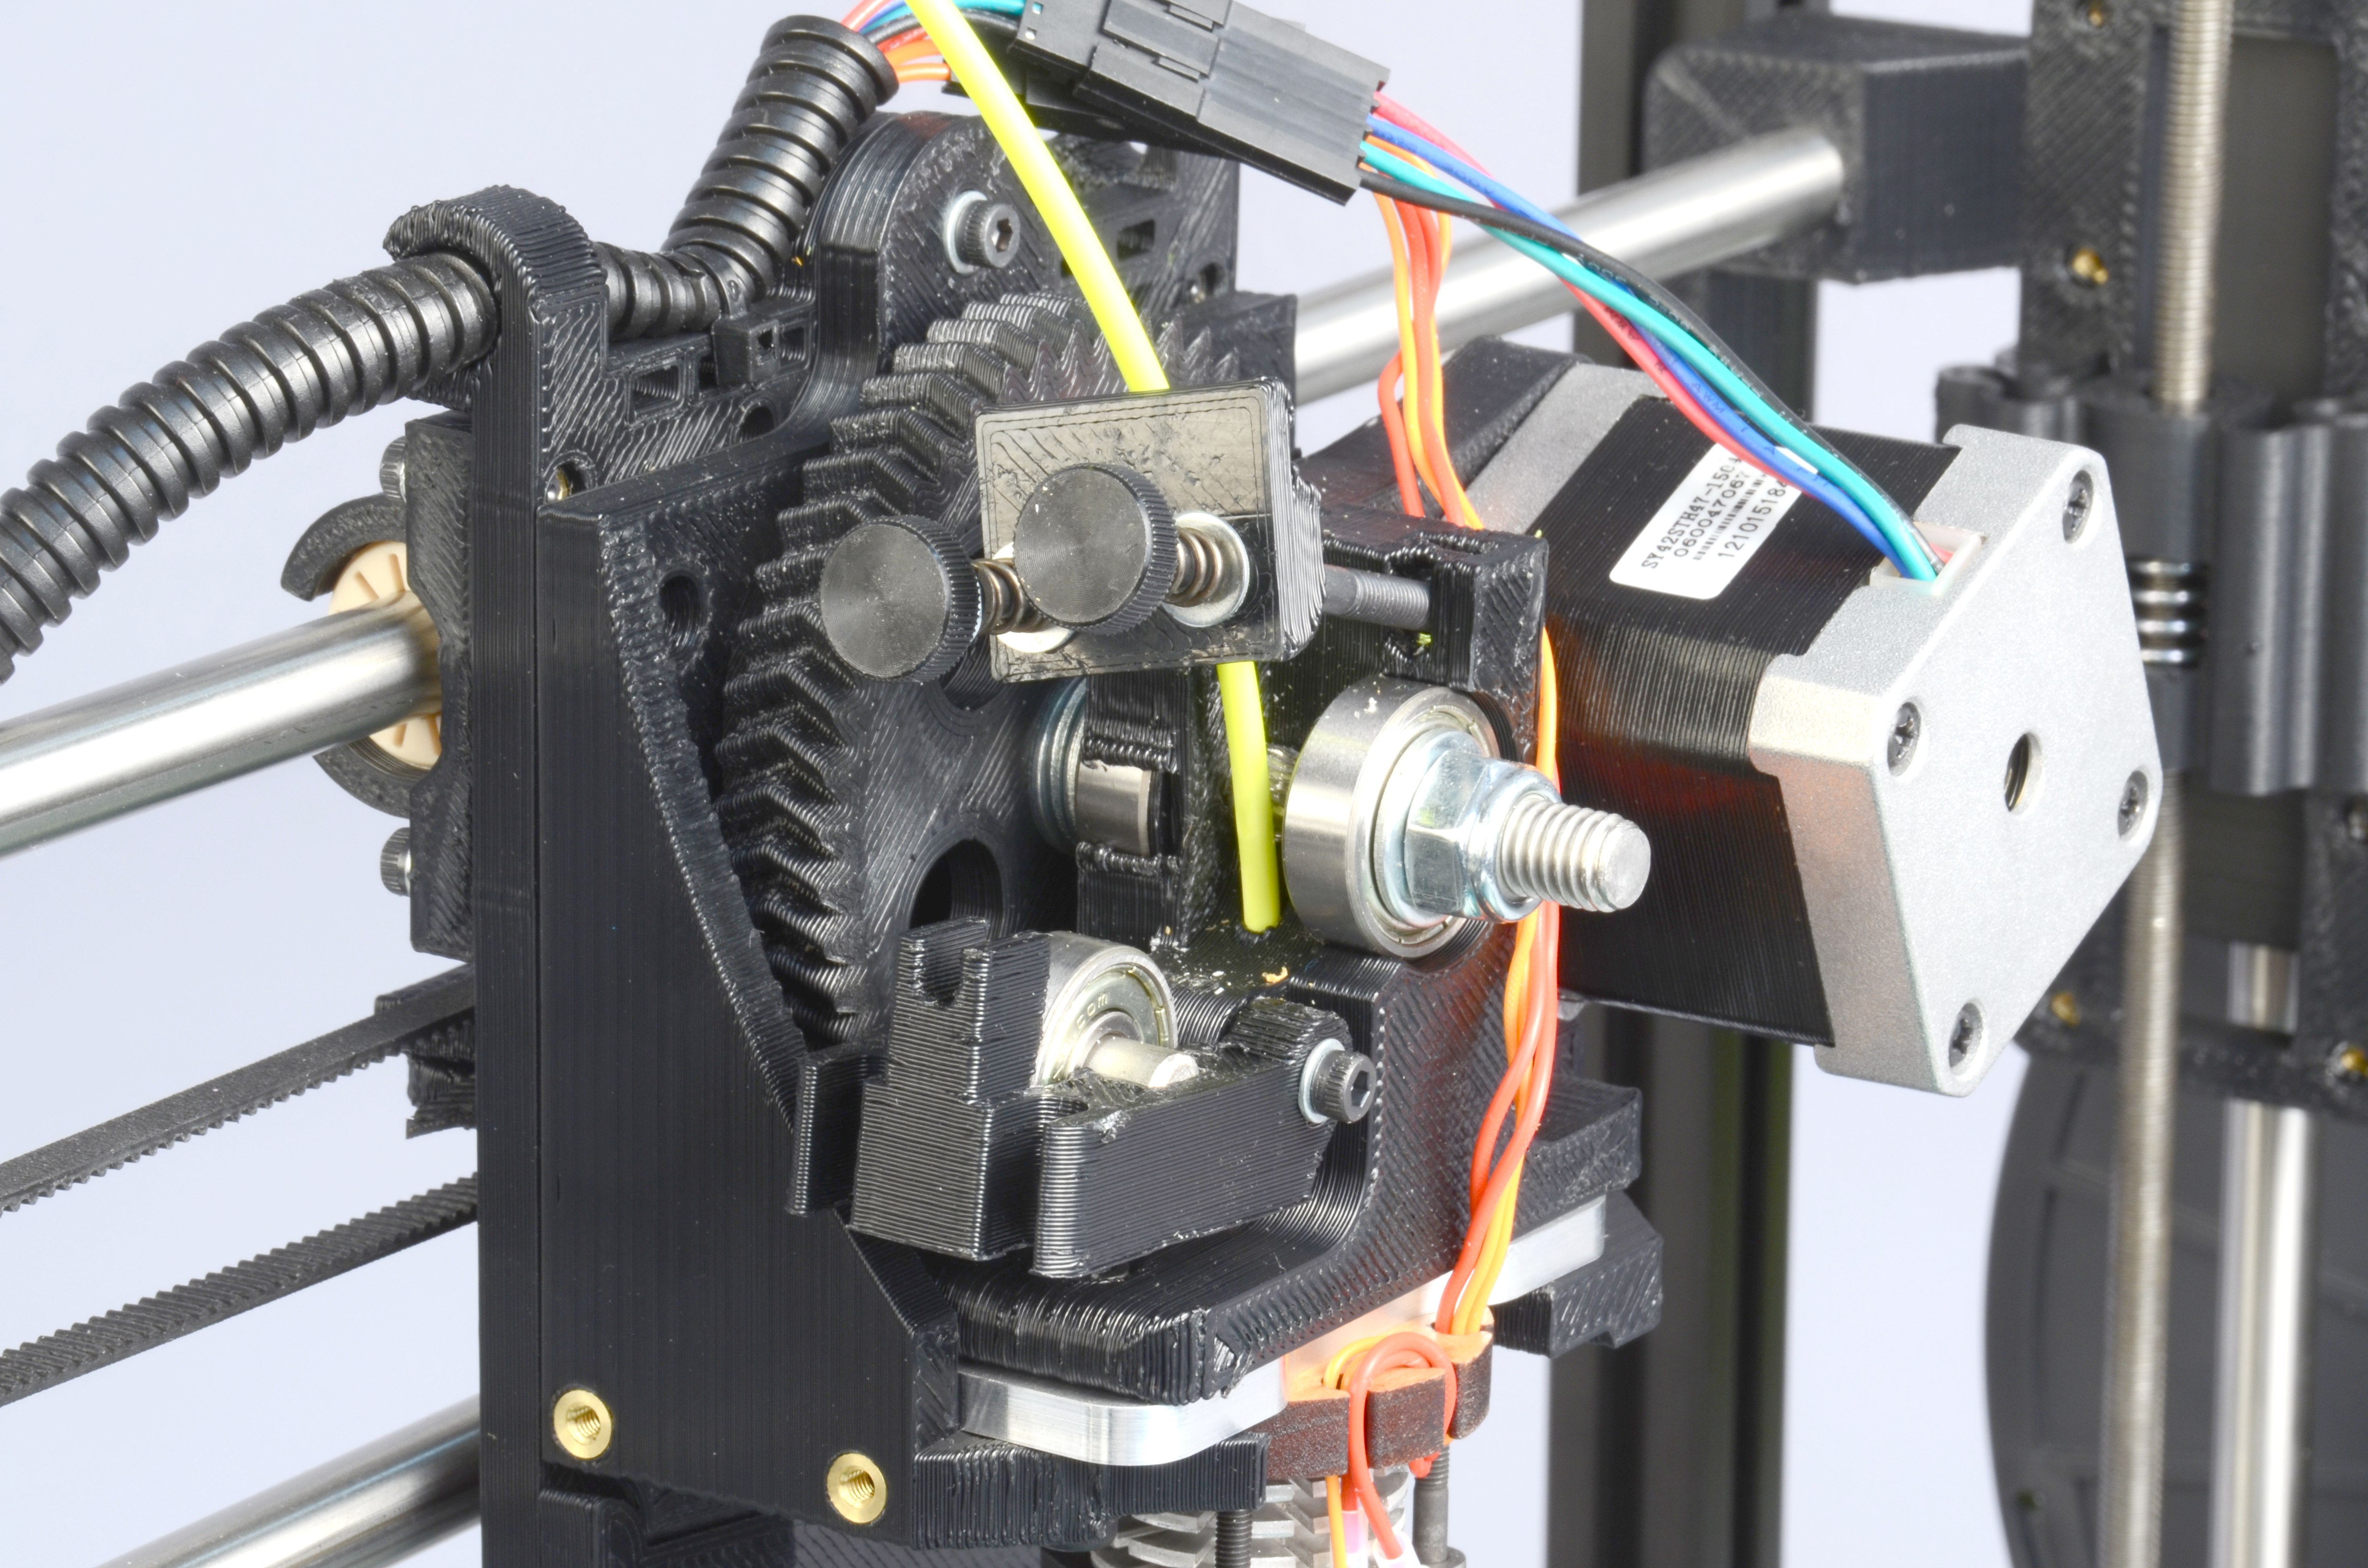
\includegraphics[keepaspectratio=true,angle=0,height=0.4\textheight,width=1.0\textwidth]{extruder_filament_slot.JPG}
\caption{Extruder filament slot}
\label{fig:extruder_filament_slot}
\end{figure}
Now you can push the filament through the extruder by slowly pushing the filament down into the hot end.

Once the filament extrudes a small amount out of the nozzle by manually pushing the filament into the extruder body raise the idler and slide the two idler bolts and plate back into place. Tighten the two idler bolts if you previously loosened them. Tighten the two screws until they are finger tight, then tighten them slightly more, until the top of the thumbscrews are about 10mm away from the plastic clip. In Pronterface, in the lower left hand corner of the screen there are two text entry boxes next to the "Extrude" and "Reverse" buttons. In the top text entry box (length in mm) change the 5 to 40. In the lower box (Speed in mm/min) change the 300 to 250. Now use the \texttt{Extrude} button in Pronterface to test that the extruder is working properly. You may need to extrude 40-60mm of filament to fully prime the hot end. Slowly tighten the two extruder thumbscrews while extruding until you achieve reliable, repeatable extrusion. If the extrusion stalls you may need to open the extruder and trim off any filament with a chewed out section.

\section{Home Printer}
Use the home buttons to home the X axis and then the Y axis. Next home the Z axis. When the Z axis is at home the nozzle tip should be right above the glass
(Fig. \ref{fig:nozzle_height}, page \pageref{fig:nozzle_height}). The image to the left, in figure \ref{fig:nozzle_height}, is the correct nozzle height.
\begin{figure}[p]
\centering
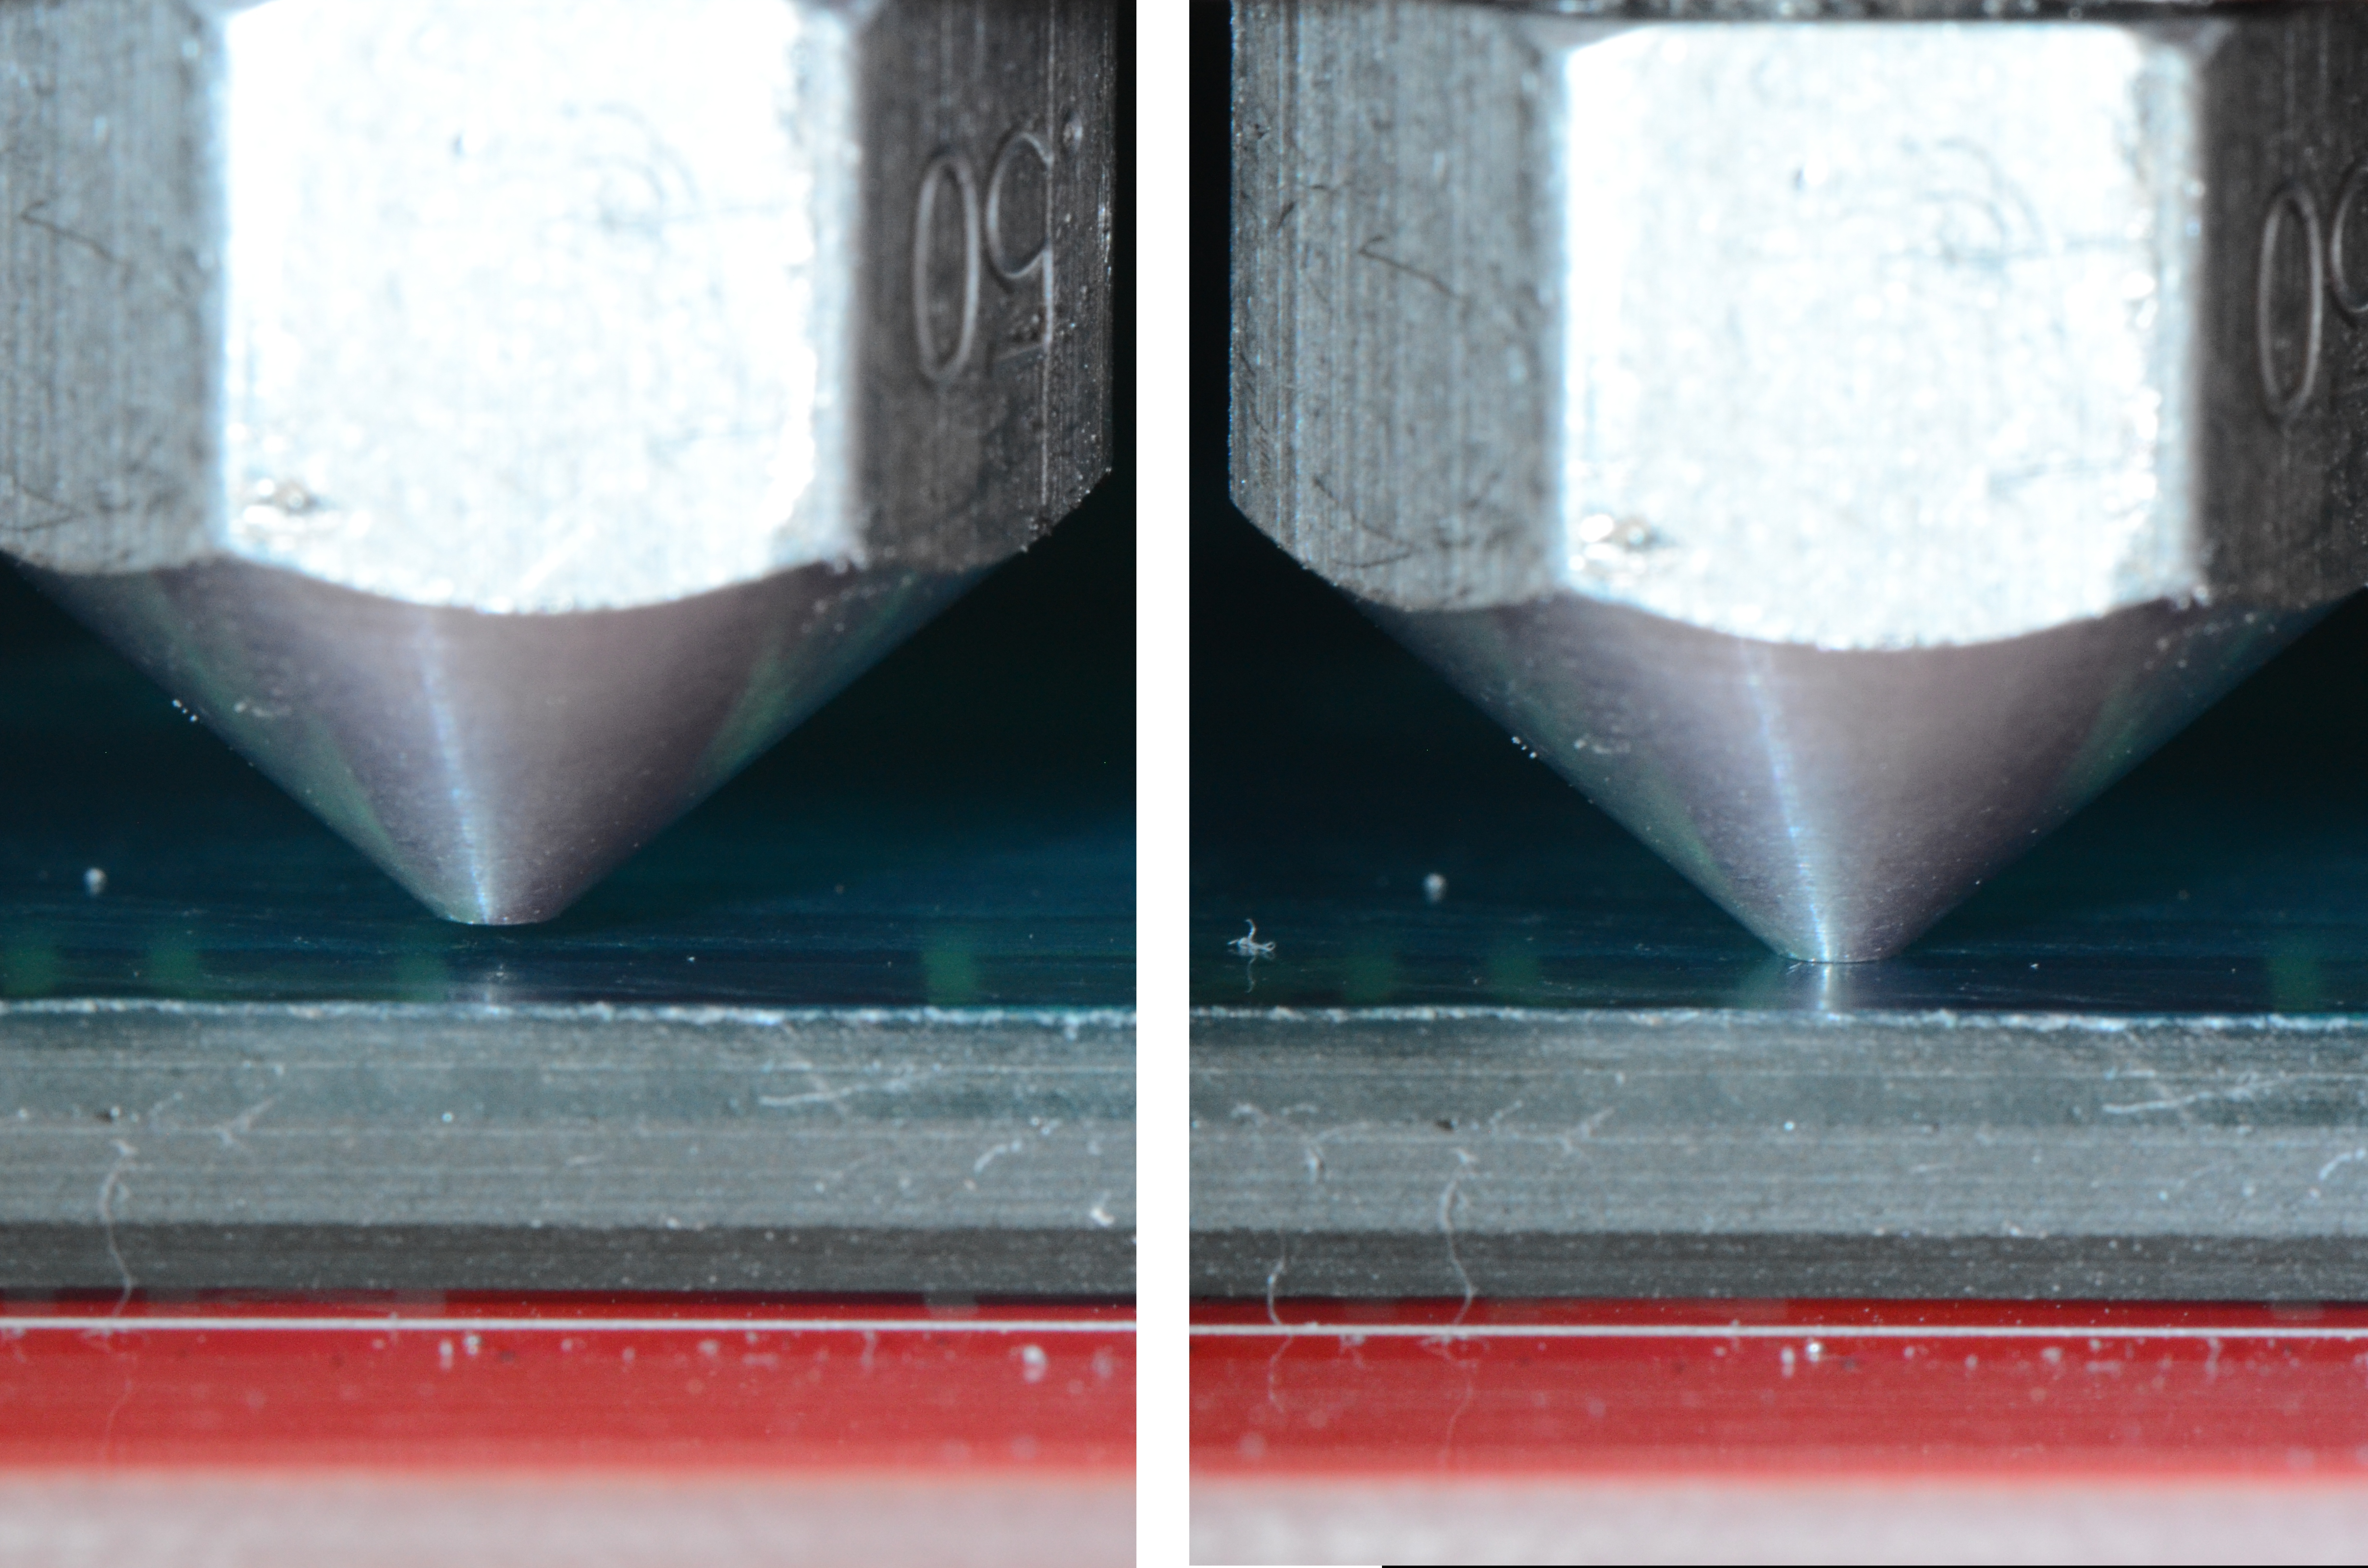
\includegraphics[keepaspectratio=true,angle=0,height=0.4\textheight,width=1.0\textwidth]{nozzle_height.jpg}
\caption{Nozzle height}
\label{fig:nozzle_height}
\end{figure}
\begin{figure}[p]
\centering
\includegraphics[keepaspectratio=true,angle=0,height=0.4\textheight,width=1.0\textwidth]{Z_end_stop_trigger.JPG}
\caption{Z end stop trigger}
\label{fig:Z_end_stop_trigger}
\end{figure}
The nozzle should not be pushing down on the print surface. To lower or raise the Z home height adjust the Z end stop trigger. The red end stop trigger is on the far left of the printer mounted on the X-axis motor mount.
(Fig. \ref{fig:Z_end_stop_trigger}, page \pageref{fig:Z_end_stop_trigger}).
The red end stop trigger can be lowered by turning clockwise and raised by turning counter-clockwise. Once you have homed the axes and the hot end and bed have reached the correct temperature it is time to print!

%fix image positioning, images for 5.3 get shoved underneath 5.4
\section{Z Print Height}
Load the \texttt{bed\_level.gcode} file.
This file can be found in the calibration directory on the SD card included with your TAZ 3D printer or at: \texttt{http://www.LulzBot.com/support/downloads}. Place your mouse cursor over the entry \texttt{Bed Level Check}, right click and select \texttt{Save as}} Once you have downloaded the file to your computer, press the \texttt{Load file} button in Pronterface. Navigate through the file browser to the downloaded \texttt{bed\_level.gcode} file, highlight the file and select the \texttt{Open} button.

The .gcode file should appear in the Pronterface G-Code viewer. Press the \texttt{Print} button to begin the print. When the print starts make sure the first layer is not printing too close or too far from the print bed. Note 
Figure \ref{fig:1st_layer_adhesion}, page \pageref{fig:1st_layer_adhesion},
\begin{figure}[hbt]
\centering
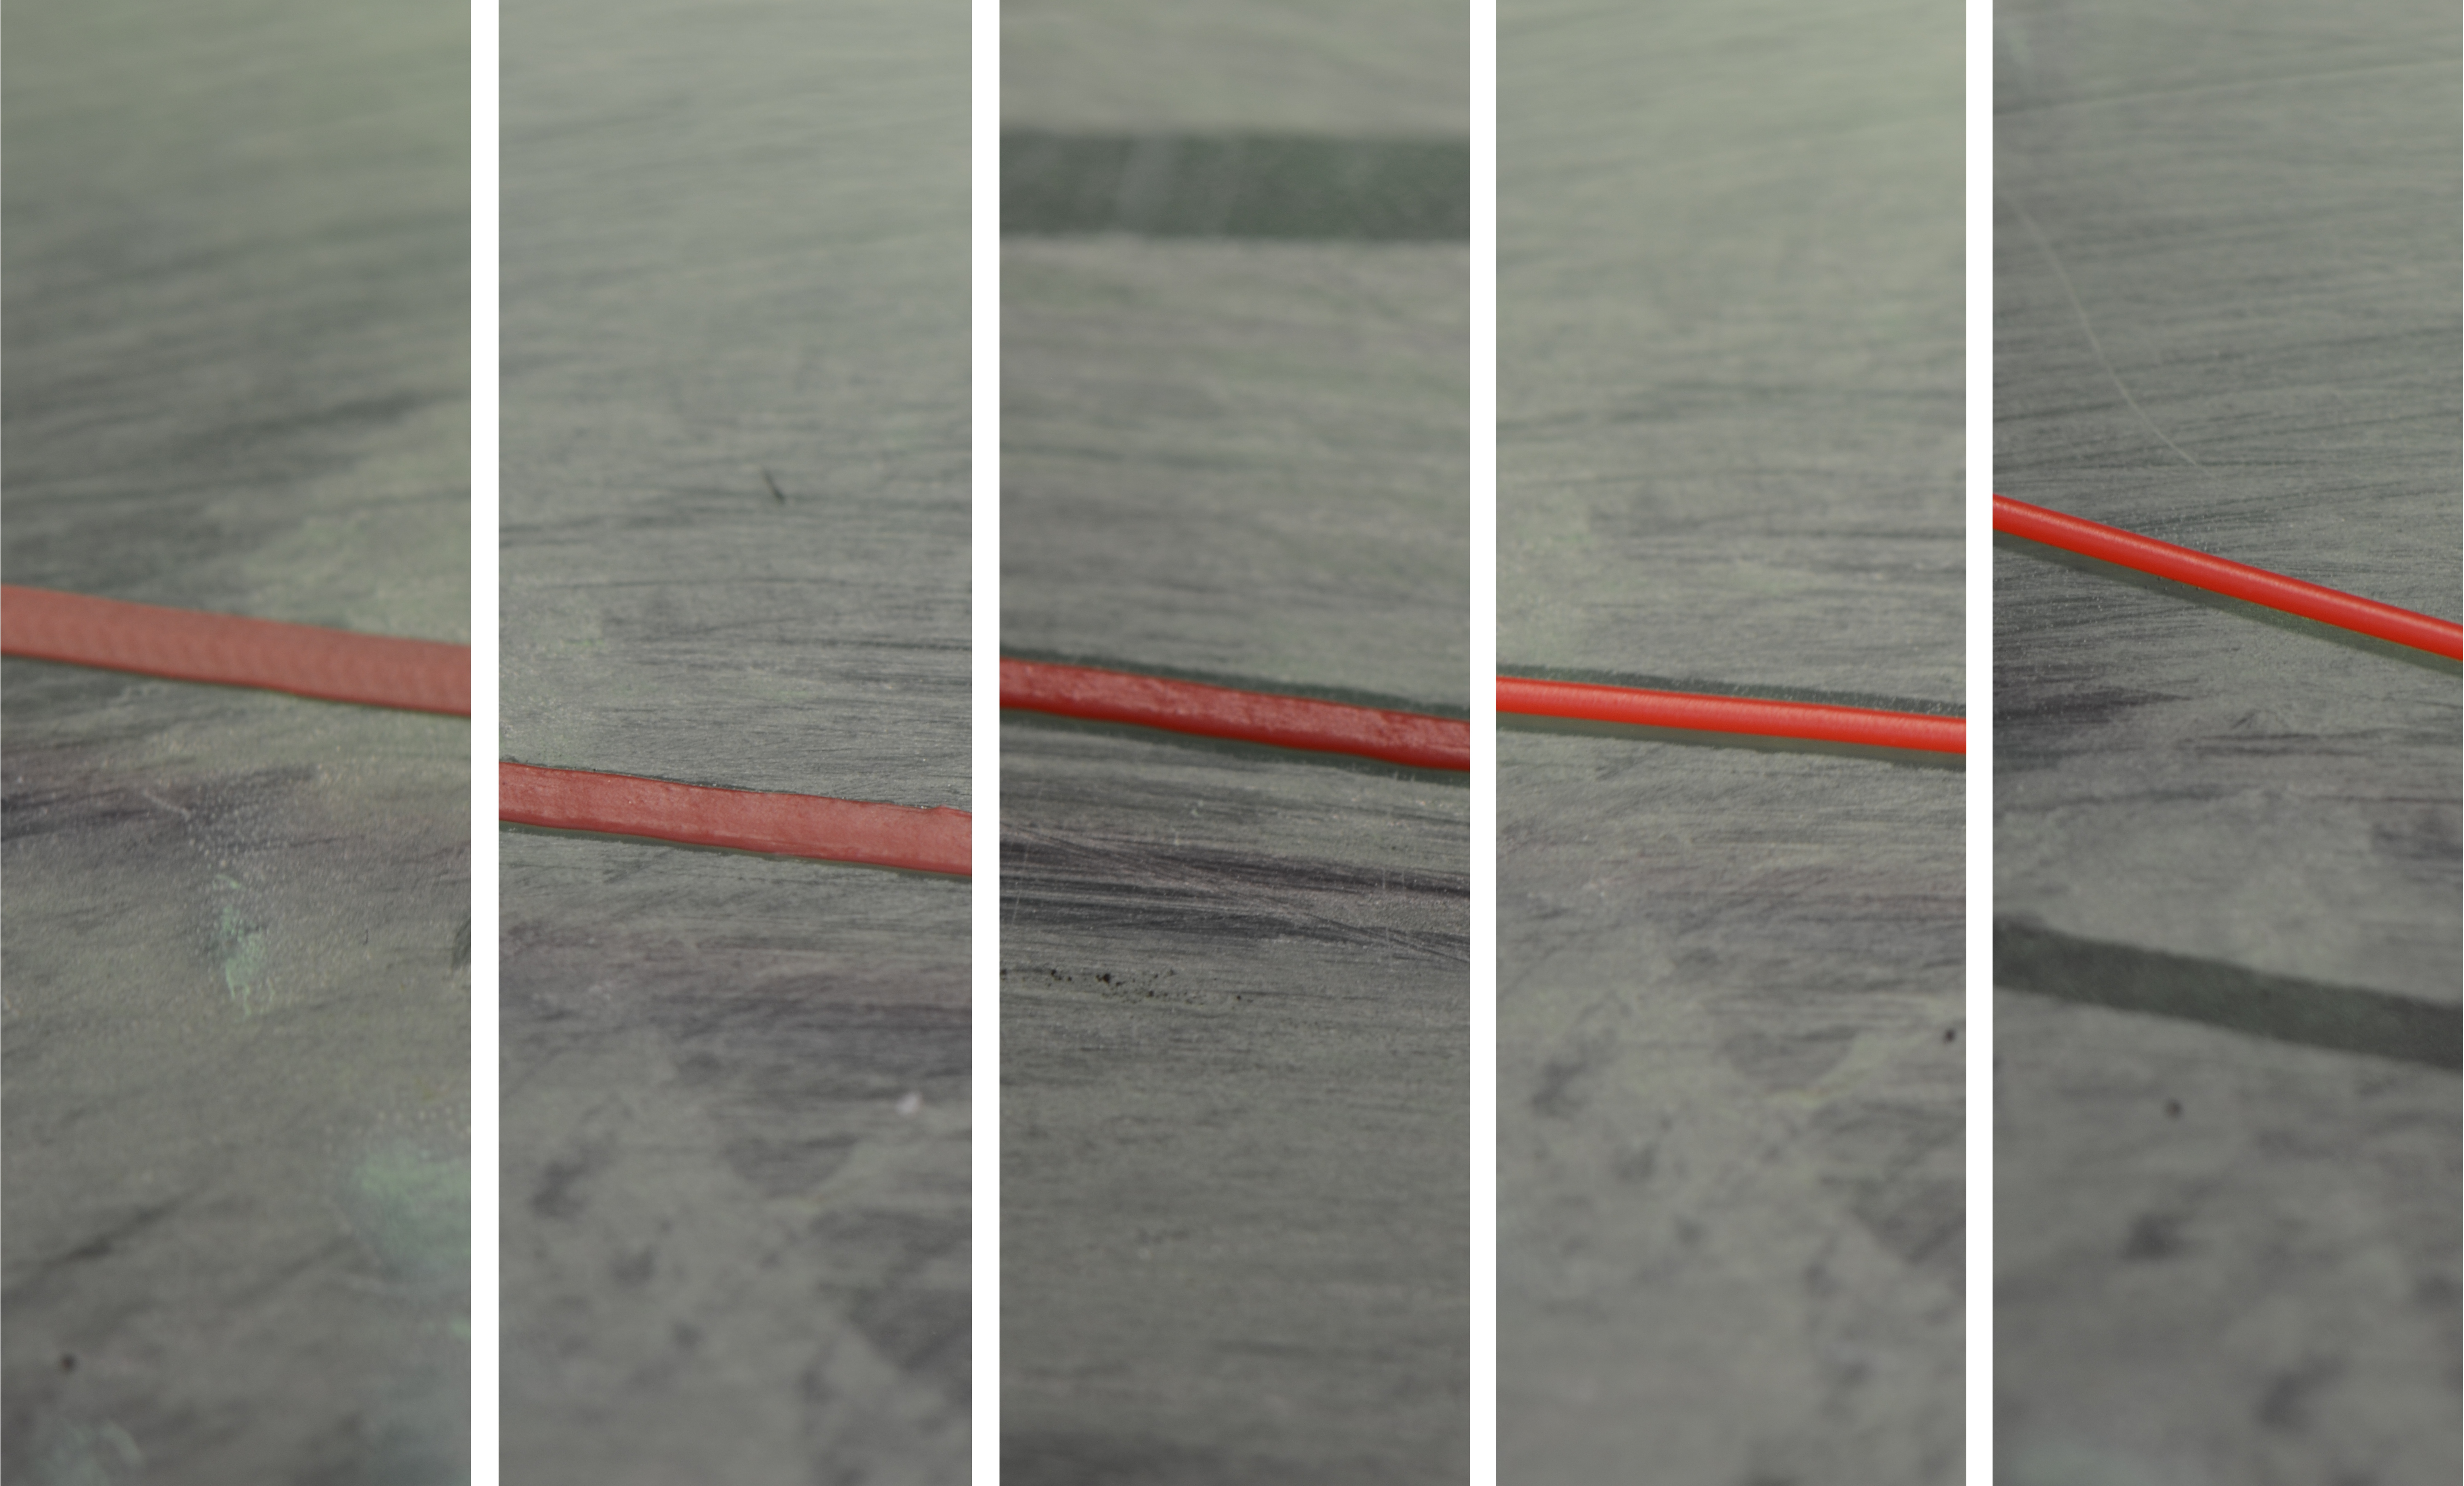
\includegraphics[keepaspectratio=true,angle=0,height=0.4\textheight,width=1.0\textwidth]{1st_layer_adhesion.jpg}
\caption{First layer adhesion}
\label{fig:1st_layer_adhesion}
\end{figure}
as an example of a good first layer adhesion. From left to right: very low, low, \emph{perfect}, high, very high. If the first layer is too high or low you can pause the print by pressing the \texttt{Pause} button. Adjust the Z end stop trigger. After making adjustments remove any printed material off the bed and home the axes and press \texttt{Restart} to restart the print. Measure the extrusion width, ideally the width would be the same in all areas of the bed. You would raise/lower a corner to minimize/increase the extrusion width to match the others. Once they are all consistent, the bed is level.

\section{Your First Octopus!}
Load the \texttt{octopus.gcode} file. This file can be found at:
\texttt{http://download.lulzbot.com/TAZ/3.0/novelties/}. Load the file in Pronterface, bring the hot end \texttt{(230C ABS/185C PLA)} and the heated bed \texttt{(85C ABS/60C PLA)} up to printing temperature. Once the printer is at the appropriate temperature, press the \texttt{Print} button to begin the print.

\section{Remove Part}
After the part is finished printing, the heated bed will automatically cool down to room temperature. If you are printing PLA you will need to turn the heated bed off. Once the bed cools you can you pop the finished part off of the printed surface. To remove the printed part, use the clam knife included in your printer kit. Leather gloves are suggested to protect your hands from the clam knife blade. It is also safe practice to not place your hand in the direction you are pushing the clam knife. Using the side of the clam knife blade pry up one side of the printed part. If your part is large you may need to pry at multiple points to pop the part off of the print surface. When removing parts take caution to not damage the PET film. If the film is cut or ripped it will peel from the glass and need to be replaced. Make sure to reset the heated bed to the correct temperature and allow it to heat up to the needed temperature before starting the next print.

